\documentclass[11pt,a4paper,twoside,openright]{report}

\usepackage[top=25mm,bottom=25mm,right=25mm,left=30mm,head=12.5mm,foot=12.5mm]{geometry}
\let\openright=\cleardoublepage

\usepackage[a-2u]{pdfx}
\catcode30=12

\usepackage[
   backend=biber
%  ,style=iso-authoryear
  ,style=numeric
  ,citestyle=numeric
  ,sortlocale=cs_CZ
  ,bibencoding=UTF8
  %,block=ragged
]{biblatex}
\addbibresource{references.bib}

%% Přepneme na českou sazbu, fonty Latin Modern a kódování češtiny
\usepackage[czech]{babel}
\usepackage{lmodern}
\usepackage[T1]{fontenc}
\usepackage{textcomp}
\usepackage[utf8]{inputenc}

% Set fonts
\RequirePackage[osf]{mathpazo} % Palatino with oldstyle figures
\newcommand\liningnums[1]{\fontfamily{ppl}\selectfont#1}
\RequirePackage{eulervm}
\RequirePackage[scaled=.8819]{sourcecodepro} % Source Code Pro typeface for monospace

%%% Další užitečné balíčky (jsou součástí běžných distribucí LaTeXu)
\usepackage{amsmath}        % rozšíření pro sazbu matematiky
\usepackage{amsfonts}       % matematické fonty
\usepackage{amsthm}         % sazba vět, definic apod.
\usepackage{bm}             % tučné symboly (příkaz \bm)
\usepackage{graphicx}       % vkládání obrázků
\usepackage{fancyvrb}       % vylepšené prostředí pro strojové písmo
\usepackage{fancyhdr}       % prostředí pohodlnější nastavení hlavy a paty stránek
\usepackage{icomma}         % inteligetní čárka v matematickém módu
\usepackage{dcolumn}        % lepší zarovnání sloupců v tabulkách
\usepackage{booktabs}       % lepší vodorovné linky v tabulkách
\makeatletter
\@ifpackageloaded{xcolor}{
   \@ifpackagewith{xcolor}{usenames}{}{\PassOptionsToPackage{usenames}{xcolor}}
  }{\usepackage[usenames]{xcolor}} % barevná sazba
\makeatother
\usepackage{multicol}       % práce s více sloupci na stránce
\usepackage{caption}
\usepackage{enumitem}
\usepackage{lipsum}
\usepackage{wrapfig}
\setlist[itemize]{noitemsep, topsep=0pt, partopsep=0pt}
\setlist[enumerate]{noitemsep, topsep=0pt, partopsep=0pt}
\setlist[description]{noitemsep, topsep=0pt, partopsep=0pt}
\usepackage{pdfpages}

\usepackage{tocloft}
\setlength\cftparskip{0pt}
\setlength\cftbeforechapskip{1.5ex}
\setlength\cftfigindent{0pt}
\setlength\cfttabindent{0pt}
\setlength\cftbeforeloftitleskip{0pt}
\setlength\cftbeforelottitleskip{0pt}
\setlength\cftbeforetoctitleskip{0pt}
\renewcommand{\cftlottitlefont}{\Huge\bfseries}
\renewcommand{\cftloftitlefont}{\Huge\bfseries}
\renewcommand{\cfttoctitlefont}{\Huge\bfseries}

% vyznaceni odstavcu
\parindent=0pt
\parskip=11pt

% zakaz vdov a sirotku - jednoradkovych pocatku ci koncu odstavcu na prechodu mezi strankami
\clubpenalty=1000
\widowpenalty=1000
\displaywidowpenalty=1000

% nastaveni radkovani
\renewcommand{\baselinestretch}{1.20}

% nastavení hlavy a paty stránek
\fancyhf{}
\renewcommand{\chaptermark}[1]{\markboth{#1}{}}
\fancyhead[RO,LE]{\leftmark}
\fancyfoot[RO,LE]{\thepage}
%\renewcommand{\footrulewidth}{0pt}
\fancypagestyle{plain}{%
\fancyhf{} % clear all header and footer fields
\fancyfoot[RO,LE]{\thepage}
\renewcommand{\headrulewidth}{0pt}
%\renewcommand{\footrulewidth}{0.5pt}
}

% Tato makra přesvědčují mírně ošklivým trikem LaTeX, aby hlavičky kapitol
% sázel příčetněji a nevynechával nad nimi spoustu místa. Směle ignorujte.
\makeatletter
\def\@makechapterhead#1{
  {\parindent \z@ \raggedright 
   \Huge\bfseries \thechapter. #1
   \par\nobreak
   \vskip 20\p@
}}
\def\@makeschapterhead#1{
  {\parindent \z@ \raggedright 
   \Huge\bfseries #1
   \par\nobreak
   \vskip 20\p@
}}
\makeatother

% Trochu volnější nastavení dělení slov, než je default.
\lefthyphenmin=2
\righthyphenmin=2

% Zapne černé "slimáky" na koncích řádků, které přetekly, abychom si
% jich lépe všimli.
\overfullrule=1mm

%% Balíček hyperref, kterým jdou vyrábět klikací odkazy v PDF,
%% ale hlavně ho používáme k uložení metadat do PDF (včetně obsahu).
%% Většinu nastavítek přednastaví balíček pdfx.
\hypersetup{unicode}
\hypersetup{breaklinks=true}
\hypersetup{hidelinks}

%%% Prostředí pro sazbu kódu, případně vstupu/výstupu počítačových
%%% programů. (Vyžaduje balíček fancyvrb -- fancy verbatim.)

\DefineVerbatimEnvironment{code}{Verbatim}{fontsize=\small, frame=single}



\def\NazevPrace{Univerzální sériový programátor}
\def\Trida{R8.A}
\def\AutorPrace{Petr Šícho}
\def\DatumOdevzdani{25.3.2022}

% Vedoucí práce: Jméno a příjmení s~tituly
\def\Vedouci{Bc. Emil Miler}

% Studijní program a obor
\def\StudijniProgram{studijní program}
\def\StudijniObor{studijní obor}

% Text čestného prohlášení
\def\Prohlaseni{Prohlašuji, že jsem svou práci vypracoval samostatně a použil jsem pouze prameny a literaturu
uvedené v~seznamu bibliografických záznamů. Nemám žádné námitky proti zpřístupňování této práce v~souladu se
zákonem č. 121/2000 Sb. o~právu autorském, o~právech souvisejících s~právem autorským a
o~změně některých zákonů (autorský zákon) ve znění pozdějších předpisů.}

% Text poděkování
\def\Podekovani{%
Chtěl bych poděkovat především open hardware komunitě, specificky pak Arduino komunitě, na jejíchž fórech jsem našel značné množství informací. Dále děkuji Bc. Emilovi Milerovi za pomoc při vedení této maturitní práce.
}

% Abstrakt česky
\def\Abstrakt{%
Tato maturitní práce si klade za cíl zjednodušit proces programování a nahrávání kódu do mikrokontrolérů v pouzdře DIP. Univerzální sériový programátor (USP), který v rámci této práce vznikl, je zařízení, které je schopné automaticky detekovat rozložení vývodů čipu vloženého do ZIF patice. Na základě toho rozpozná o který mikrokontrolér se jedná a uzpůsobí pro něj nahrávací obvod. Teoreticky by měl USP umět programovat všechny mikrokontroléry pracující na napětí 5 voltů a podporovat dostatečně pomalé bit-banging programovací protokoly, včetně těch, které vyžadují vysoké napětí (12V) pro resetování. Aktuálně je implementována podpora rodin ATtiny a ATmega od výrobce Atmel. Na softwarové úrovni USP pracuje na protokolu Arduino ISP.
}

% Abstrakt anglicky
\def\AbstraktEN{%
This thesis aims to simplify the process of programming and uploading code to microcontrollers in a DIP package. The Universal Serial Programmer (USP), which was created in this work, is a device that is able to automatically detect the distribution of terminals on a chip inserted into the ZIF socket. Based on this, it recognizes which microcontroller is present and adapts the programming circuit for it. Theoretically, the USP should be able to program all microcontrollers operating at 5 volts and supporting sufficiently slow bit-banging programming protocols, including those that require high voltage (12V) for reset. A support is current implemented for the ATtiny and ATmega families from the manufacturer Atmel. At a software level, the USP is working on the Arduino ISP protocol. 
}

% 3 až 5 klíčových slov
\def\KlicovaSlova{programátor, mikrokontrolér, AVR, nahrávač, USP}
% 3 až 5 klíčových slov anglicky
\def\KlicovaSlovaEN{programmer, microcontroller, AVR, uploader, USP}


\begin{document}

%%% Titulní strana práce a další povinné informační strany

%%% Titulní strana práce

\pagestyle{empty}
\pagenumbering{gobble}
\hypersetup{pageanchor=false}

\begin{center}
\LARGE
\textbf{GYMNASIUM JANA KEPLERA}\\
{\large Parléřova 2/118, 169 00 Praha 6}

\vspace{\stretch{3}}


\includegraphics[width=.3\textwidth]{img/logo}

\vspace{\stretch{3}}

{\Huge\bfseries\NazevPrace}

\vspace{8mm}
\mdseries{Maturitní práce}

\vspace{\stretch{8}}
\large
\begin{tabular}{rl}
Autor: & \AutorPrace \\
\noalign{\vspace{2mm}}
Třída: & \Trida\\
\noalign{\vspace{2mm}}
Školní rok: & 2021/2022\\
\noalign{\vspace{2mm}}
Předmět: & Informatika \\
\noalign{\vspace{2mm}}
Vedoucí práce: & \Vedouci \\
\end{tabular}

\vspace{20mm}
Praha, \DatumOdevzdani
\end{center}


\openright

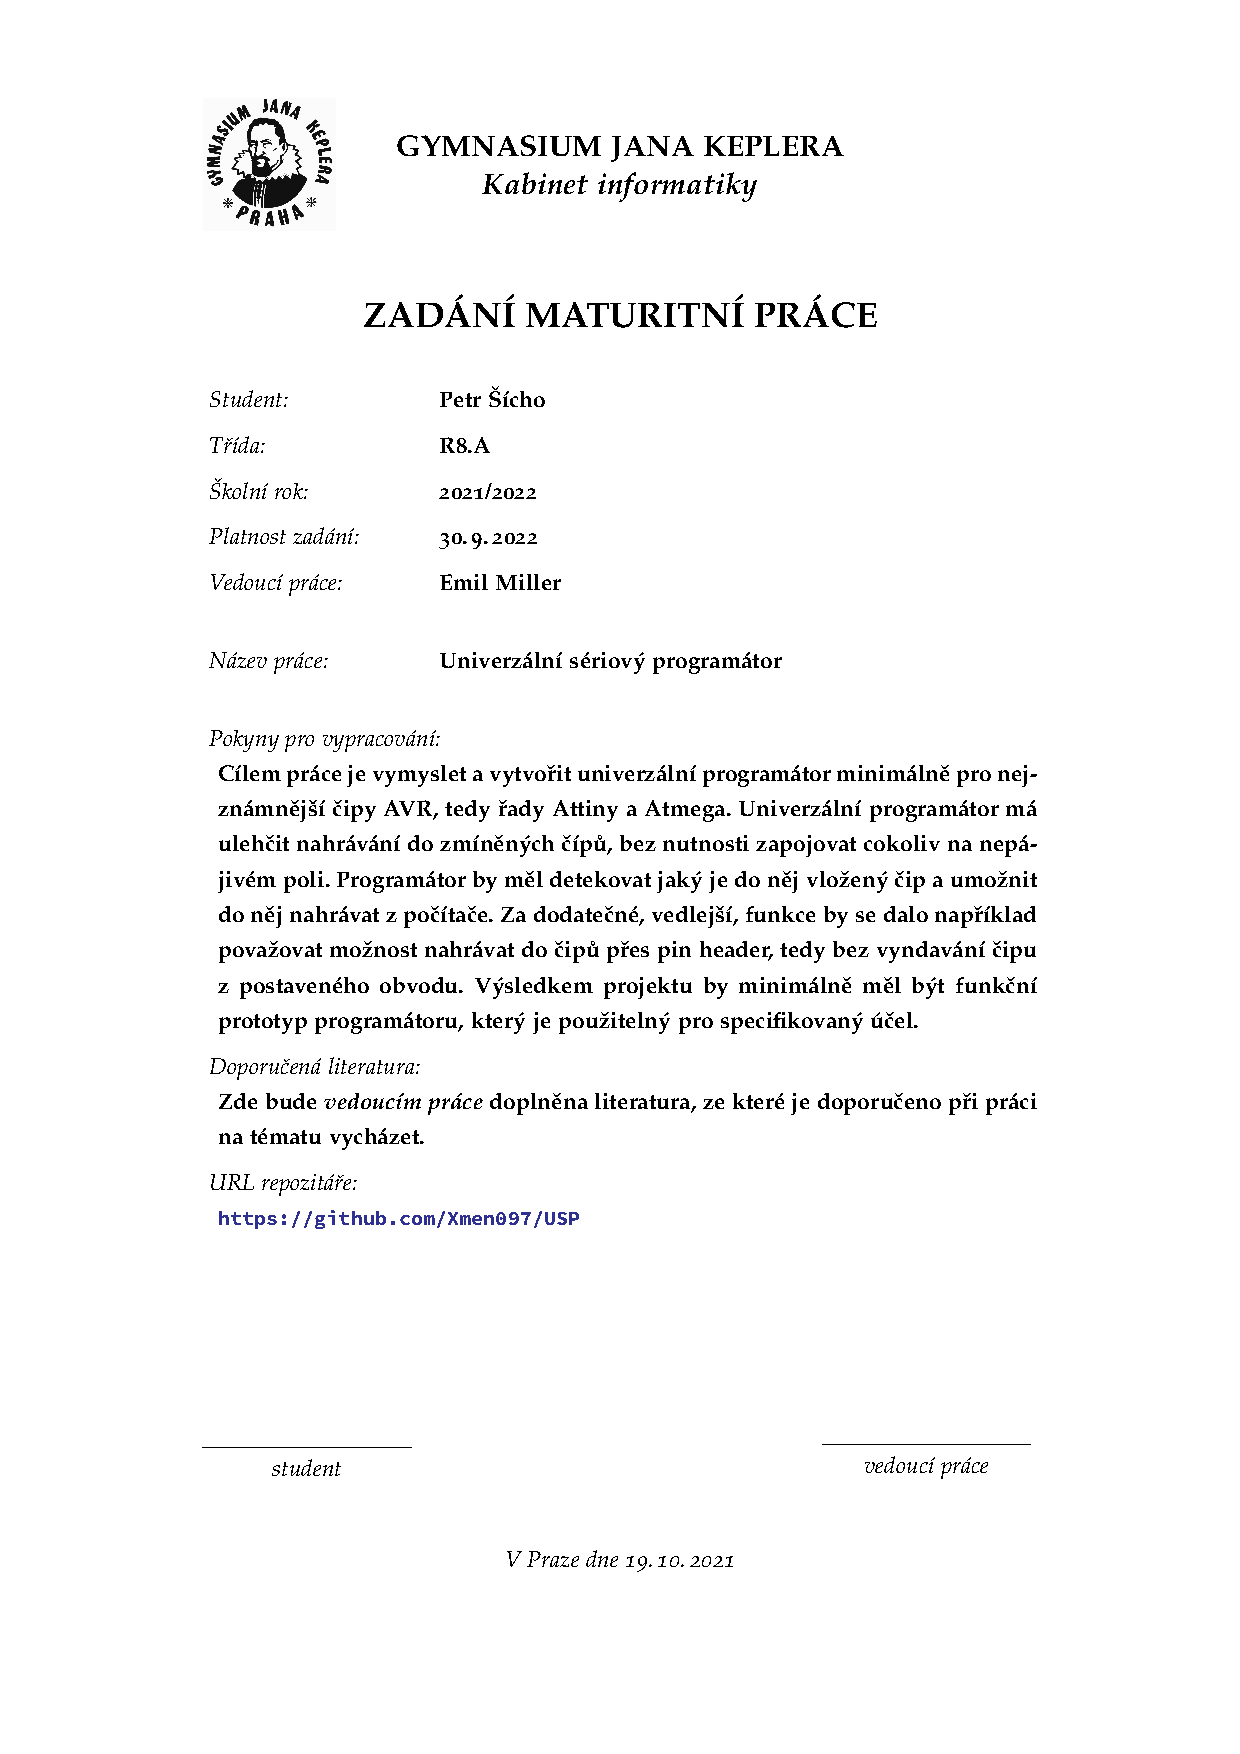
\includepdf[]{zadani.pdf}


%%% Strana s čestným prohlášením k bakalářské práci

\hypersetup{pageanchor=true}
\cleardoublepage
\vspace*{\fill}
\section*{Prohlášení}
\noindent
\Prohlaseni

\vspace{2cm}
\noindent
V Praze dne \today
\hspace*{\fill}\small{\AutorPrace}
\vspace{1cm}

%%% Poděkování
\openright
\vspace*{\fill}
\section*{Poděkování}
\noindent
\Podekovani
\vspace{1cm}


%%% Povinná informační strana bakalářské práce
\openright
\section*{Abstrakt}
\noindent
\Abstrakt
\subsection*{Klíčová slova}
\noindent
\KlicovaSlova

\vfill

\section*{Abstract}
\noindent
\AbstraktEN
\subsection*{Keywords}
\noindent
\KlicovaSlovaEN

\openright
\pagenumbering{arabic}

% Obsah
\setcounter{tocdepth}{2}
\tableofcontents

\chapter{Teoretická část}
\pagestyle{fancy}

Existuje nepřeberné množství různých čipů a s nimi podobné množství různých rozložení vývodů, které nejsou jednotné ani u jedné velikosti a jednoho výrobce. Pro každé rozložení pinů mikrokontroléru je nutné mít externí programovací obvod. Cílem práce je sjednotit tyto programovací obvody do jednoho univerzálního, který se přizpůsobí vloženému čipu. Fungování USP lze rozdělit na dvě části - detekovat čip a následně umožnit jeho programování. 

Pro univerzální programátor není možné použít žádný dedikovaný hardware, který by zajišťoval nahrávání. Naopak je vhodné použítí univerzálních vstupních~/~výstupních pinů neboli GPIO\footnote{z anglického General-purpose input/output, tedy pin, který se umí chovat buď jako digitální vstup, nebo výstup, přičemž mezi těmito módy je možné přepínat.} pinů. I přes snahu o maximální univerzálnost není reálné docílit podpory úplně všech existujících čipů. Jako minimální požadovanou funkcionalitu jsem tedy bral podporu čipů AVR od výrobce Atmel, konkrétně pak řady ATmegy a ATtiny, které zahrnují mikrokontroléry, jež pohání známé desky Arduino. Přesto se domnívám, že vlastnosti těchto čipů, na kterých je detekce a nahrávání postaveno, budou do velké míry přenositelné i na jiné rodiny či výrobce čipů.

\section{Detekce}

Základem detekce je poznat jak velký čip je - tedy kolik má vývodů. Tím bychom mohli v prvním přiblížení detekce radikálně omezit počet potenciálních kandidátů. Při zahrnutí jen několika modelů, jednoho pro každou velikost, bychom tak měli detekci téměř hotovou. Bylo by však nutné arbitrárně stanovit tyto podporované čipy, přičemž při vložení jiného, ať třeba ze stejné rodiny, který má prohozené piny GND a VCC, by došlo pravděpodobně k jeho zničení. Naší ambicí tedy bude zjistit o čipu co nejvíce informací, díky nimž budeme schopni rozeznávat mezi co největším počtem různých čipů.

Při detekci si musíme dávat pozor, abychom náhodou mikrokontrolér nepoškodili. Ideálně bychom se chtěli držet v hodnotách, které povoluje jeho datasheet. Problém je, že to, o co se pokoušíme, není standardní zacházení s čipy a v datasheetu tak nenalezneme konkrétní povolené hodnoty a situace, kterým můžeme čip bezpečně vystavit. Z datasheetu vybraných AVR čipů \cite{attiny85, atmega328, atmega2560, attiny84} můžeme alespoň určit některé společné zásady, kterých když se budeme držet, tak minimalizujeme poškození čipu. Konkrétně se jedná o:
\begin{itemize}
	\item Nevystavovat žádný pin napětí nižšímu než $-0.5V$
	\item Nevystavovat žádný pin, kromě RESETu, napětí vyššímu než ${V}_{cc} + 0.5V$
	\item Nevystavovat RESET napětí vyššímu než $13V$
	\item Nenechat mezi žádný dvěma piny nezapojeného čipu téct nezanedbatelně velký proud po nezanedbatelně dlouhou dobu\footnote{Pro naše účely budeme považovat za zanedbatelný proud řádu mikroampér a čas mikrosekund.}
\end{itemize}
Při splnění těchto podmínek by měl být čip dostatečně chráněn obvody, které běžně slouží k ochraně před elektrostatickým výbojem (ESD). 

\subsection {Detekce velikosti a polohy \label{theory:capacitance}}

Pro detekci velikosti čipu můžeme využít toho, že každá reálná součástka, kromě svých primárních vlastností, vykazuje také elektrickou kapacitu. To bude jistě platit i pro spoje a součástky uvnitř integrovaných obvodů. Elektrická kapacita pinů jednoduchých CMOS\footnote{Complementary metal-oxide semiconductor; technologie výroby integrovaných obvodů.} čipů \cite{multiplexer, switch2, switch1} se pohybuje v jednotách pikofaradů. Není mi znám žádný způsob přímého měření elektrické kapacity, budeme tedy muset provést měření nepřímé a dostatečně přesné. Jednou z možností je kapacitor pomalu nabíjet nebo vybíjet a měřit čas, který k tomu budeme potřebovat. Zkusíme odhadnout jak přesné takové měření bude s pomocí rovnice definující energii elektrického kondenzátoru \begin{equation} E = \frac{1}{2}CU^2 \end{equation}
Budeme-li kapacitor nabíjet napětím $U$ a proudem $I$ po dobu $t$, můžeme psát
\begin{equation} {W}_{max} = U \cdot I \cdot t \end{equation} 
Jedná se o horní odhad vykonané práce, která počítá s nulovým odporem a nulovým elektrickým potenciálem kapacitoru. Reálná energie předaná kapacitoru bude nižší, což nám však nevadí. Úpravou těchto dvou vztahů můžeme vyvodit úměrnost
\begin{equation} C \simeq t / R \end{equation}

Zjistili jsme, že kapacita je přímo úměrná času, po který jsme kapacitor nabíjeli, a nepřímo úměrná odporu, přes který jsme nabíjeli.\footnote{Ke stejnému výsledku bychom došli i použitím rozměrové analýzy.} Čas budeme schopni měřit velice přesně\footnote{Přesnost měření času je omezena frekvencí oscilátoru řídícího mikrokontroléru, běžně se pohybuje v desítkách megahertzů.}, řádově v mikrosekundnách ($10^{-6} s $). Řekněme, že pin čipu má kapacitu $10 pF = 10^{-11} F$. Dosazením do vztahu (1.3) zjistíme, že k jejímu změření budeme potřebovat nabíjecí odpor o velikosti $100 k\Omega$. To nebude problém, měření vypadá proveditelně.

Díky schopnosti změřit kapacitu na každém z pinů socketu zjistíme nejenom jak velký čip je, ale zároveň i kde v socketu je vložen. Není tedy nutné nijak specifikovat na jakou pozici v socketu má být čip pro nahrávání vložen.

\subsection {Detekce speciálních pinů}

Každý mikrokontrolér má kromě vstupních~/~výstupních pinů i speciální piny, které plní nějakou zvláštní funkci. Například je to RESET pin, napájecí piny (GND a VCC) nebo piny hodin (XTAL). Tyto piny by mohly vykazovat rozdílné elektrické vlastnosti a možná i rozdílnou kapacitu. Vzhledem k tomu, že napájecí piny jsou vnitřně připojené k všemožným součástem mikrokontroléru, lze hlavně u těchto pinů očekávat vyšší kapacitu. Tu bychom při dostatečně přesném měření kapacity detekovat a rozpoznat tak polohu napájecích pinů.

\subsection {Rozpoznání VCC od GND\label{VCCvsGND}}

Při špatném rozpoznání vloženého mikrokontroléru může největší poškození způsobit převrácení pinů GND a VCC. Abychom se tohoto rizika vyvarovali, je nutné rozpoznávat s jistotou VCC od GND. Tím zároveň obecně snížíme šanci na špatné rozpoznání čipu.

Využijeme ochranných diod, které jsou připojeny ke každému IO pinu mikrokontroléru, jak ukazuje obrázek \ref{fig:pin_diagram}. Povšimněme si, že dioda spojující pin s GND směřuje opačně, než dioda spojující pin s VCC. Díky tomu bychom měli být schopni rozpoznat, zda je určitý pin GND či VCC.

\begin{figure}[ht!]
  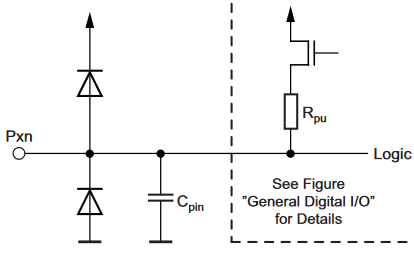
\includegraphics[width=0.4\textwidth]{img/pin_diagram.png}
  \centering
  \caption{Schéma vnitřního zapojení IO pinu mikrokontroléru \cite[str.~58]{atmega328}.}
  \label{fig:pin_diagram}
\end{figure}

Pin GND můžeme detekovat následovně. Budeme znát úbytek napětí na diodě mezi pinem a GND $U_d$. Přivedeme-li na pin GND napětí $U$ převyšující $U_d$, měli bychom na všech IO pinech detekovat napětí $U-U_d$. Z bezpečnostních důvodů by napětí $U$ by mělo být co nejmenší možné, ideálně $U<0.5V$. Napětí přivedeme přes dostatečně velký odpor tak, aby mikrokontrolérem a diodou tekl co nejmenší proud. S malým procházejícím proudem budeme mít také menší úbytek napětí na diodě (menší, než běžně udávaných $\sim0.7V$)

Obdobným způsobem je možné detekovat pin VCC. Stačí na libovolný (nebo lépe postupně na všechny) IO pin přivést napětí $U$ a na pinu VCC by se nám vždy mělo ukázat napětí $U-U_d$.

\subsection {Závěr}

S touto výbavou bychom měli být schopni dostatečně detailně rozpoznat mikrokontroléry ATmega a ATtiny. Díky rozpoznáním GND a VCC budeme schopni čip bezpečně napájet. Nebude pak problém, kdybychom chtěli rozšířit podporované čipy a vyskytly by se nám dva čipy, které mají na stejných místech GND a VCC, ale na různých místech piny potřebné pro nahrávání. V této situaci bychom postupně vyzkoušeli různá rozložení nahrávacích pinů, až bychom našli to správné.

\section {Nahrávání}

Po detekování čipu nám už zbývá pouze do něj nahrát. Vzhledem k tomu, že přesně nevíme jaké rozložení pinů bude čip mít, musíme použít tzv. bit-banging\footnote{Softwarová implementace určitého protokolu, která přímo generuje protokolem specifikovaný signál, bez použití specializovaného hardwaru.}. Díky tomu se nemusíme při stavbě hardwaru nahrávače omezovat na určité čipy, ale budeme schopni teoreticky obsluhovat všechny čipy, které nevyžadují příliš velké komunikační rychlosti\footnote{Maximální rychlost komunikace je tím, jak rychle jsme schopni zpracovávat odchozí a příchozí data.} a existuje pro ně bit-banging implementace nahrávání. Nebude tak ani obtížné obměňovat nahrávací protokoly pro různé čipy nebo situace.

Komplikací může být, že některé nahrávací protokoly vyžadují použití vyššího napětí. U AVR čipů jde konkrétně o protokoly HVSP (high voltage serial programming) a HVPP (high voltage parallel programming), které se hodí při určitém nastavení mikrokontroléru, kdy není možné standardní programování.\footnote{Jde např. o situace kdy je vypnuté resetování pomocí RESET pinu, protože ho chceme použít na jinou funkci.} Vysokým napětím je v obou případech myšleno 12 voltů \cite{AVRprog}. Vzhledem k tomu, že ve valné většině případů lze programovat mikrokontrolér bez použití vysokého napětí, bral jsem jeho dostupnost spíše jako bonus než nutný požadavek. High-voltage programováním se tedy budeme zabývat pouze z hardwarového hlediska.

\section {Shrnutí požadovaných funkcí\label{pinFunc}}

V této sekci si shrneme funkce, které budeme potřebovat pro úspěšnou detekci a nahrávání do čipů. Těmito funkcemi by měl disponovat každý z pinů socketu, neboť nevíme, kde se zrovna čip ocitne. Některé funkce budou komplexní (přečti kapacitu připojenou k pinu), u jiných se bude jednat o nějaký elementární stav (připojení k zemi/5V). 

\begin{enumerate}
\item \textbf{5V s proudem >20 mA} je potřeba pro napájení čipu. Proud 20 mA by měl stačit pro napájení AVR čipů \cite{attiny85, atmega328}. Některé větší čipy za určitých okolností mohou mít spotřebu větší než 20 mA, ale mají také více separátních napájecích pinů, mezi které se proud rozloží \cite[str.~286-323]{atmega32}.
\item \textbf{0V (GND) s proudem >20 mA} je potřeba též pro napájení čipu. 
\item \textbf{5V s libovolně malým proudem} reprezentuje logický stav 1 při komunikaci, odebíraný proud během komunikace bude zanedbatelný.
\item \textbf{0V (GND) s libovolně malým proudem} reprezentuje logický stav 0 při komunikaci.
\item \textbf{Čtení digitální hodnoty} pro čtení odpovědi čipu při nahrávání; standardní funkce GPIO pinů.
\item \textbf{Přečtení kapacity} pro detekci čipu.
\item \textbf{Napětí přibližně 0.4-0.5V} je potřeba pro rozpoznání GND a VCC, viz sekce \ref{VCCvsGND}.
\item \textbf{Přečtení napětí na pinu} je také potřeba pro rozpoznání GND a VCC.
\item \textbf{12V} bude potřeba pokud budeme chtít high-voltage programování.
\item \textbf{Nepřipojeno} k ničemu. Piny, které nevyužíváme k jiné funkci, by se měly chovat tak, jako kdyby nebyly k ničemu připojené.
\end{enumerate}


%%% IMPLEMENTACE


\chapter{Implementace}

Implementace projektu měla dvě fáze. Nejprve bylo potřeba navrhnout hardwarovou část - vymyslet a vyzkoušet jednotlivé části obvodu tak, aby plnily požadované funkce. Poté bylo potřeba všechny spojit do jednoho celku, který se vyrobí jako plošný spoj. Po osazení plošného spoje součástkami a otestování základní funkčnosti následoval vývoj softwaru. Jako první probíhala implementace low-level komunikace s jednotlivými součástkami, pak přišly na řadu high-level funkce detekce. 

Pojďme si nyní jednotlivé fáze rozebrat detailněji.

\section {Hardware}

Převážná část práce na hardwaru probíhala s pomocí nepájivého pole, na kterém jsem postupně testoval jednotlivé ideje uvedené v teoretické části práce. V následujících sekcích si rozebereme jaké součástky byly použity a jak se pomocí nich implementují požadované funkce ze sekce \ref{pinFunc}.

\subsection {Vkládání čipu}

Jako patici, do které se bude vkládat čip k programování, jsem zvolil ZIF (zero insertion force) socket. Jak již jméno napovídá, pro vložení čipu do patice není nutné užití síly. Stačí čip položit na patici a pomocí páčky na straně patice čip zajistit, čímž vznikne spolehlivý kontakt s piny čipu. Nehrozí tak ohnutí nožiček čipu a jeho vložení i vyndání je velmi rychlé. Nevýhodou ZIF socketu je o trochu vyšší pořizovací cena a větší velikost, ale i přesto se v našem případě určitě vyplatí. Konkrétně jsem zvolil patici se 40 piny (dvaceti na každé straně), která by měla postačovat pro naprostou většinu DIP\footnote{Dual in-line package; pouzdro s THT piny s roztečí 2.54mm.} pouzder. Patice podporuje vložení jak úzké (0.3''), tak široké (0.6'') varianty DIP.

\subsection {Řídící mikroprocesor}

Je potřeba zvolit mikroprocesor, který bude ovládat celý nahrávač. Volil jsem mezi mikrokontroléry AVR, s kterými jsem nejvíce obeznámen a které také umí jednoduše komunikovat s Arduino IDE. Zásadní otázkou je kolik budeme potřebovat GPIO pinů k ovládání USP. Určitě bude potřeba jeden pin pro každý pin ZIF patice, tedy minimálně 40 pinů. Další desítky pinů budou potřeba pro ovládaní komponent a součástek, o kterých se budu detailněji zmiňovat v dalších sekcích. Teoreticky by bylo možné přidat další piny pomocí shift registrerů či IO expanderů. Tím by však utrpěla rychlost komunikace a vzrostla by komplexita desky a tím i prostor pro chyby. Rozhodl jsem se tedy pro jeden co největší čip, mikrokontrolér ATmega2560 v pozdře TQFP100, který má 84 GPIO pinů \cite{atmega2560}.

Nejprve jsem plánoval, že bych využil dostupných schémat Arduino desek a v upravené podobě je přímo zakomponoval do desky nahrávače. To by umožnilo využít řídící čip bez omezení. Na druhou stranu by tím extrémně vzrostla komplexita desky a také celková cena. Nakonec jsem se tedy rozhodl programátor vyvinout jako shield (nasazovací desku) na Arduino Mega s mikroprocesorem ATmega2560. Nevýhodou tohoto postupu může být snad jen to, že Arduino mega nám dává k dispozici pouze 70 z 84 GPIO pinů, ale i to by mělo pro tento projekt stačit \cite{ArduinoMega}.

\subsection {Základní funkcionalita pinů}

Nyní přichází na řadu implementace požadovaných funkcí popsaných v sekci \ref{pinFunc}. Jenom tím, že ke každému pinu ZIF socketu bude připojený GPIO pin, zajistíme funkce 3, 4, 5, které GPIO piny zvládají nativně. Funkce 1 a 2, které vyžadují minimální proud 20 mA, také s trochou opatrnosti zvládneme. Digitální piny ATmegy2560 dokáží dodávat maximální proud 40 mA \cite[str.~355-356]{atmega2560}. Musíme tedy jen dát pozor na to, aby další součástky, které budou zapojeny mezi GPIO pinem a pinem ZIF socketu neměly příliš velký odpor nebo nevyžadovaly více omezený protékající proud.

Desátý požadavek vyžaduje trochu zamyšlení. Pin určitě nebude možné fyzicky odpojit, to bychom museli provést manuálně. Budeme tedy alespoň chtít minimalizovat proud, který může skrz tento \lq odpojený\rq   pin téct. Když nastavíme GPIO pin jako vstupní, bude ve stavu s tzv. vysokou impedancí, tedy poteče jím malý proud. Datasheet specifikuje maximální proud jako $1 \mu  A$, typický proud lze očekávat výrazně menší \cite[str.~355]{atmega2560}. Odpojení si navíc můžeme pojistit použitím analogového přepínače, u kterého je udáván maximální proud $100nA$ a typický $0.05nA$ \cite[str.~3]{switch1}.

\subsection {Zapojení multiplexerů}

Implementaci funkcí 6, 7, 8 a 9 si zjednodušíme pozorováním, že v jednu chvíli bude daná funkce potřebná pouze na jednom pinu. Nemusíme ji tedy implementovat 40x, ale můžeme použít multiplexery k spojení určitého pinu s něčím, co nám funkci zajistí. Napětí na pinu budeme číst pomocí ADC\footnote{Analogově digitální převodník; zařízení, které převede analogový signál (napětí) v určitém rozsahu na digitální tvar s určitým počtem bitů, v našem případě se jedná o převodník 10-bitový.} převodníku. Atmega2560 disponuje jedním ADC převodníkem, který je ale vnitřně multiplexován na 16 GPIO pinů. Pomocí dalších multiplexerů rozšíříme tuto funkcionalitu na všech 40 pinů.

%Pro zajištění správného přečtení napětí nemůžeme nechat ADC převodník tzv. floating, tedy nepřipojený k ničemu, kdy vrací víceméně náhodné hodnoty. Všech 5 ADC pinů, které využíváme, je tedy připojeno rezistorem $1M\Omega$ k zemi. Takto vysokou hodnotu rezistoru jsem volil, aby se nezkreslily výsledky měření kapacity.

Multiplexery se standardně vyrábí s $2^n$ kanály, které se ovládají pomocí $n$ pinů. Zvolil jsem 8 kanálové multiplexery \cite{multiplexer}, tedy s 3 ovládacími piny. Pro obsluhu 40 pinů jich bude potřeba celkem 5. Multiplexery jsou připojeny k pinům ZIF socketu způsobem znázorněným na obrázku \ref{fig:mux_diagram}.

\begin{figure}[ht!]
  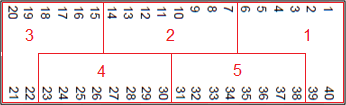
\includegraphics[width=0.4\textwidth]{img/mux_diagram.png}
  \centering
  \caption{Schéma zapojení mulitplexerů k pinům ZIF patice.}
  \label{fig:mux_diagram}
\end{figure}

Díky tomuto způsobu zapojení budeme schopni odhalit závadu na multiplexeru při rozpoznávání čipu, neboť i nejmenší mikrokontrolér, který má pouzdro DIP8 se 4 piny na každé straně, bude mít vždycky alespoň dva piny v různých multiplexerech. Nestane se tedy, že by kvůli závadě na jednom multiplexeru (ta může být způsobená i třeba dotekem uživatele, kterým se zvýší kapacita) byl čip chybně rozpoznán.

\subsection {Napěťový dělič \label{voltage_divider}}

Napětí 0.4-0.5V, jak si žádá sedmý požadavek, vytvoříme pomocí napěťového děliče. Zde se nám budou hodit již výše zmíněné multiplexery. Dělič napětí bude totiž právě mezi GPIO pinem a multiplexovaným pinem. Na každém GPIO pinu je možné zapnout tzv. pullup rezistor, který pin připojí přes odpor s přibližnou velikostí $30-40k\Omega$\footnote{Datasheet udává, že odpor bude vždy větší než $20k\Omega$ a menší než $50k\Omega$. Vzhledem k tomu, že tyto hodnoty jsou pro teplotní rozmezí od -55°C do 125°C můžeme konstatovat, že při pokojové teplotě bude odpor přibližně mezi $30-40k\Omega$.} k 5 voltům. Kýžené napětí přibližně půl voltu vytvoříme dalším rezistorem s velikostí $3.3k\Omega$\footnote{Chceme dělič napětí přibližně 1:10, hodnotu odporu jsem zvolil o něco nižší, protože i samotný multiplexer bude mít určitý odpor (asi 100 ohmů).} k zemi. Zapojení děliče napětí na pinu je vidět na obrázku \ref{fig:voltage_divider}


\begin{figure}[ht!]
  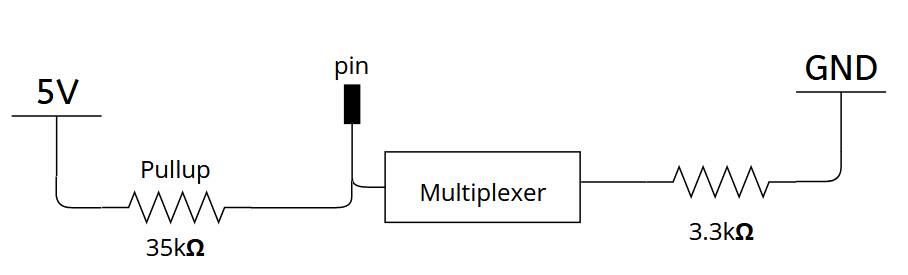
\includegraphics[width=0.6\textwidth]{img/voltage_divider.png}
  \centering
  \caption{Schéma děliče napětí.}
  \label{fig:voltage_divider}
\end{figure}

\subsection{Měření kapacity}

Kapacitu lze měřit, jak jsme vyvodili v sekci \ref{theory:capacitance}, pomocí pomalého nabíjení - tedy nabíjení přes dostatečně velký rezistor. Vypočítali jsme, že by se nám hodil rezistor s odporem $100k\Omega$. Připojovat takový odpor k pinům by si však vyžádalo dalších multiplexerů nebo switchů. Můžeme ale využít stejných pullup rezistorů, které využíváme pro napěťový dělič. Ty jsou o něco menší a mohlo by se stát, že kapacitor nabijeme příliš rychle. Můžeme ale využít ADC převodníku, který máme multiplexovaný k pinům. Původně jsme chtěli měřit čas, za který nabijeme plně kapacitor, což bychom zjišťovali pomocí digitálního vstupu GPIO pinů. Můžeme to ale provést i opačně. Kapacitor budeme nabíjet nějaký konstantní čas, a poté pomocí ADC převodníku zjistíme napětí na kapacitoru. Čím vyšší napětí bude, tím více jsme kapacitor nabili a tím je tedy kapacitor menší. Opačně by šlo i kapacitor plně nabít a poté ho nechat samovolně vybíjet. Počkáme konstantní čas a opět pomocí ADC převodníku zjistíme, jak moc se vybil. 

Při testování se ukázalo, že pro měření kapacity se nám velmi hodí i dělič napětí, podrobněji viz sekce \ref{software:capacitance}

\subsection {Napětí 12 voltů\label{12v}}

Poslední funkcionalitou, kterou nám zbývá implementovat je dostupnost napětí 12 voltů. To můžeme na pin pouštět pomocí stejných multiplexerů, které využíváme k připojení ADC převodníku. Stačí pomocí switche CD4066B \cite{switch2} přepínat zdroj multiplexeru mezi 12 volty a ADC převodníkem. Zapojení tohoto obvodu pro multiplexer 1 a 2 je vyobrazeno v příloze  \ref{appendix:mux_input_control}. Od použitého switche nepožadujeme žádné zvýšené nároky ohledně proudu, pro HVSP i HVPP nám stačí malý proud. Problém je, že náš řídící mikrokontrolér, ale ani většina dobře dostupných multiplexerů, nepodporuje vyšší napětí než 5 voltů. S trochou snahy se dají najít i multiplexery podporující 12 voltů. Řídíci čip, jehož piny odolají napětí 12 voltů, ale prakticky není možné najít. Budeme proto muset piny řídíciho mikrokontroléru odpojit předtím, než připojíme 12 voltů. K tomu využijeme analogové switche MC14066B \cite{switch1}. Vzhledem k tomu, že přes tyto switche budeme mimo jiné napájet čip, který budeme chtít programovat, musí podporovat průtok proudu alespoň $20mA$.\footnote{Z tohoto důvodu se použitý switch liší od switchů \cite{switch2}, které používáme u zdroje multiplexeru.} 

Každý switch má 4 kanály, které dokáže přepínat pomocí 4 ovládacích pinů. Není však možné ani potřebné ovládat každý z těchto pinů individuálně, na to bychom totiž spotřebovali dalších 40 pinů. Šlo by pomocí tranzistorů a odporů detekovat zvýšené napětí a přepnout ovládací pin switche. To by však vyžadovalo značné množstí externích komponent - na každý pin jeden tranzistor a několik odporů. Lepší řešení je založené na faktu, že 12 voltů bude vždy připojené na pinu, který je multiplexován. Toho využijeme a přidáme další multiplexer, který bude mít stejně zapojené ovládací piny jako první multiplexer. Bude fungovat tak, že vypne kanál, který obsluhuje pin, ke kterému je multiplexováno. Tímto zajistíme přepínání s použitím pouze jediného pinu, který bude sloužit k potlačení této funkcionality, která by nám rozbila napětový dělič a další funkce. Zjednodušené schéma tohoto systému pro 8 pinů ZIF patice je znázorněno na obrázku \ref{fig:simplified_pin_switches}. Tento obvod je na USP celkem 5 krát - pro každých 8 pinů, a to podle stejné schématu jako zapojení původních multiplexerů (obrázek \ref{fig:mux_diagram}). Kompletní zapojení toho obvodu je dostupné jako příloha \ref{appendix:pin_switches}.

\begin{figure}[ht!]
  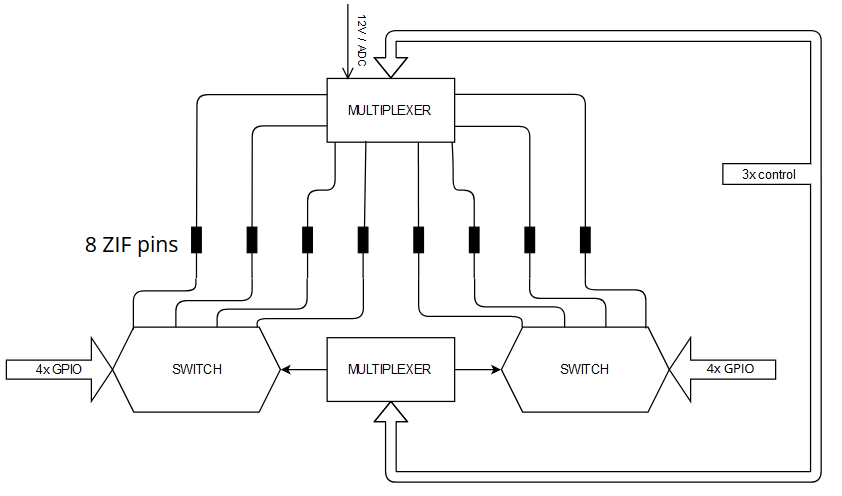
\includegraphics[width=0.8\textwidth]{img/simplified_pin_switches.png}
  \centering
  \caption{Zjednodušené schéma obvodu připojeného k 8 pinům ZIF patice}
  \label{fig:simplified_pin_switches}
\end{figure}

Další komplikací spojenou s vyšším napětím je, že multiplexery a switche potřebují být ovládané tímto napětím. Nestačí tedy již připojit na ovládací pin multiplexeru/switche GPIO pin řídícího mikrokontroléru, ale je nutné použít tranzistor a pullup/pulldown\footnote{V závislosti na tom v jakém výchozím stavu chceme, aby byl ovládací pin; ve většině případu se bude jednat o pulldown rezistor.} rezistor.

Poslední věcí, kterou musíme vyřešit, je kde získat napětí 12 voltů. Jednou možností by bylo zapojit do USP přímo toto napětí z externího zdroje, to by ale výrazně ztížilo jeho použití. Rozhodl jsem se proto přímo do USP zabudovat step-up převodník, který nám vytvoří napětí 12V. Obvod step-up převodníku byl navržen podle datasheetu regulátoru MC34063A \cite{step-up}. Celé zapojení obvodu převodníku je zobrazeno v příloze \ref{appendix:boost_converter}.

\subsection {Dodatečný hardware}

Krom výše uvedených součástek a obvodů, které slouží k zajištění detekce nebo nahrávání, je USP vybaven také 0.91'' OLED displejem a čtyřmi tlačítky. To umožní tvorbu uživatelského rozhraní pro jednodušší ovládání programátoru. OLED displej je také užitečným nástrojem pro debugování. Dále jsou pak na programátoru tři LED - modrá, zelená a červená, které slouží pro optickou signalizaci stavu programátoru.

\subsection {Využití pinů}

Nakonec se ukázalo, že 70 pinů není až zase tolik a bylo nutné s nimi trochu šetřit. Následovat bude krátký přehled toho, k čemu bylo použito kolik pinů a případně jakým způsobem byly piny uspořeny.

\begin {itemize}
\item \textbf{40 pinů} je nutných k obsloužení všech pinů na ZIF patici.
\item \textbf{5 pinů s podporou ADC} je připojeno k pěti multiplexerům.
\item \textbf{3 piny} jsou použity pro sdílenou kontrolu multiplexerů na právé straně ZIF patice (1, 2 a 3). \footnotemark{}
\item \textbf{3 piny} jsou použity pro sdílenou kontrolu multiplexerů na levé straně ZIF patice (4 a 5). \footnotemark[\value{footnote}]
\item \textbf{5 pinů} ovládá jestli je každý z pěti multiplexerů připojen k 12 voltům nebo ADC převodníku.
\item \textbf{1 pin} ovládá zda switche odpojují piny, na které je právě multiplexováno, jak je popsáno v sekci \ref{12v}.
\footnotetext{Pro všechny funkce kromě rozpoznání VCC a GND (sekce \ref{VCCvsGND}) nám stačí vždy jen jeden pin připojený k multiplexeru, ostatní multiplexery můžeme ignorovat. Pro rozpoznání VCC a GND budeme potřebovat dva multiplexery, jeden pro vytvoření malého napětí a druhý pro čtení ostatních pinů. K tomu nám ale postačí nezávisle ovládat multiplexery na jiných stranách ZIF patice, neboť díky rozložení multiplexerů podle obrázku \ref{fig:mux_diagram} bude mít i nejmenší možný čip alespoň dva piny na různých stranách.}
\item \textbf{2 piny} jsou použity pro display.
\item \textbf{4 piny} jsou využívány tlačítky.
\item \textbf{3 piny} ovládají LEDky.
\item \textbf{2 piny} jsou potřeba pro sériovou komunikaci s počítačem.
\item \textbf{zbylé 2 piny} jsou vyvedeny do headeru.
\end {itemize}

Celkem je tedy využito všech 70 dostupných pinů.

\subsection {Plošný spoj}

Po otestování částí některých výše zmíněných obvodů na nepájivém poli bylo potřeba vytvořit návrh desky plošného spoje. Rozhodl jsem se rovnou pro 4-vrstvý plošný spoj, vzhledem k tomu, že jsem plánoval umístit co nejvíce součástek na co nejmenší plochu a vrchní vrstva je tak prakticky celá pokryta ploškami pro kontakty součástek. Prostřední dvě vrstvy jsou udělány jako tzv. plane, kde většina vrstvy zabírá jeden signál, zde konkrétně země a napájení, a slouží pro snížení rušení na desce. Hotového zapojení plošného spoje je k nahlédnutí v příloze \ref{appendix:board}.

%Plošný jsou jsem si nechal vyrobit a osadit SMD součástkami u nejmenované čínské firmy. Hlavní výhodou objednání z Číny je řádově menší cena, než u ostatních výrobců, problémem na druhou stranu může být, že čínané mají často vlastní kopie součástek a jejich datasheety nejsou přeložené do angličtiny. Většinou jsou k nalezení anglické datasheety prakticky totožných součástek jiných výrobců. Po výrobení plošného spoje jsem začal zjišťovat na co vše jsem při návrhu zapomenul a co nefunguje. Naštěstí nic z toho nebylo kritické a bylo možné všechny nedostatky opravit.


%%% SOFTWARE


\pagebreak
\section {Software}

Přestože bylo cílem projektu vytvořit co nejlepší hardwarový výrobek, je jeho nedílnou součástí i software nutný k zprovoznění tohoto hardwaru. Nicméně ne všechny funkce implementované na hardwarové úrovni jsou využity ze strany softwaru. 

\subsection{Princip fungování}

Po zapnutí USP detekuje vložení čipu, který následně identifikuje a data o něm předá nahrávači (více o něm v sekci \ref{software:uploader}). Nahrávač pak vykonává příkazy, které dostane po sériové lince a programuje vložený čip, dokud uživatel nezmáčkne resetovací tlačítko. Princip fungování konkrétně zachycuje obrázek \ref{fig:app_diagram}. 

\begin{figure}[ht!]
  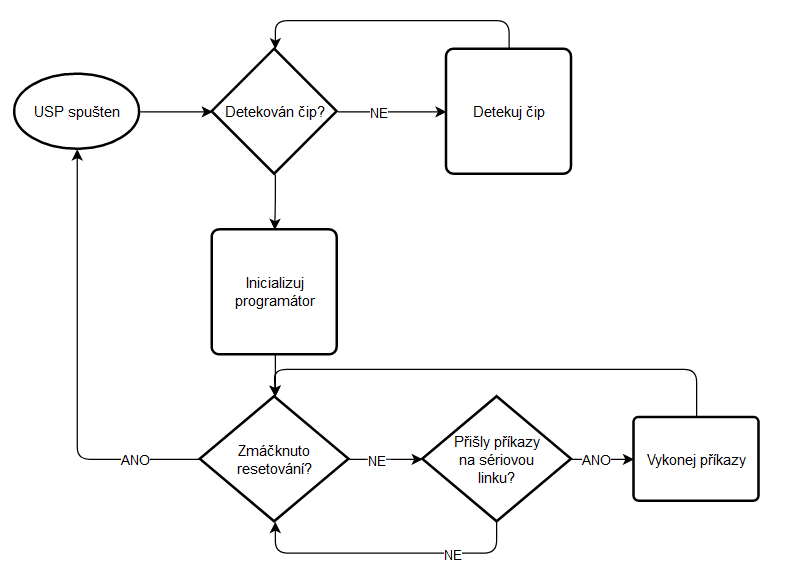
\includegraphics[width=0.75\textwidth]{img/app_diagram.png}
  \centering
  \caption{Diagram USP}
  \label{fig:app_diagram}
\end{figure}

\subsection {Nízkoúrovňové funkce}

Jako první bylo potřeba implementovat funkce pro ovládání hardwaru - konkrétně multiplexerů, OLED displeje a tlačítek. U tlačítek stačilo implementovat tzv. debouncing, tedy brát tlačítko jako stisknuté až tehdy, když se jeho stav po nějakou dobu nemění.

Pro práci s displejem jsem použil knihovnu od Adafruitu pro ovladač SSD1306, kterým je displej vybaven. Pro převod obrázků a grafik na displej jsem využil aplikaci image2cpp \cite{image2cpp}. Na displeji jsou implementovány převážně debugovací funkce, které se však mohou hodit i během provozu zařízení. Není totiž vyloučené, že měření, která bylo potřeba nakalibrovat\footnote{Měření kapacity je kalibrované pomocí aditivní a multiplikativní konstanty, které byly nalezeny experimentálně. Bez těchto úprav se kapacita na pinech výrazně lišila, pravděpodobně z důvodu rozdílné délky spojů na PCB, případně jejich vystavení působení jiných komponent.}, se budou v určitých situacích chovat trochu jinak a bude nutné je kalibrovat znovu. Z tohoto důvodu jsou kalibrační data uložena v paměti EEPROM, aby je bylo možné měnit i bez flashování.

Pro zprovoznění multiplexerů jsem použil návrhový vzor Composite, kdy každý z pěti multiplexerů je instancí třídy, která obstarává vnitřní mapování jeho ovládacích pinů na výstup a další nastavení. Všechny multiplexery jsou pak společně ovládány pomocí jiné třídy, která pozná, který multiplexer má použít.

\subsection {Interface \label{software:capacitance}}

Interface funguje jako prostředník mezi nízkoúrovňovými hardwarovými funkcemi a detektorem, kterým se bude zabývat následující sekce. Poskytuje funkce změření kapacity či napětí na pinu, připojení napětí 0.5 voltu a další.

Měření kapacity bylo implementování s přesností, která umožňuje rozpoznání polohy speciálních pinů. Prakticky měření probíhá tak, že pin nabíjíme pomocí napětí 0.5 voltů po dobu 5 mikrosekund\footnote{Tato doba při testování dávala nejlepší výsledky.}. Pak nabíjet přestaneme a změříme napětí, které na pinu je. Samotné změření napětí trvá nějaký čas, během kterého se pin stihne částečně vybít. Změřené napětí je tedy zčásti dáno rychlostí nabíjení i rychlostí vybíjení. Tento způsob měření ukázal, že piny GND a VCC mají prakticky dvojnásobnou měrnou kapacitu než normální piny. Pin RESET je také zajímavý. U některých čipů se z pohledu kapacity chová jako kdyby tam vůbec nebyl. U jiných čipů má naopak kapacitu výrazně vyšší než normální piny. V obou situacích jsme schopni pin RESET rozpoznat jako speciální pin.

\subsection {Detektor}

Detektor implementuje vysokoúrovňovou detekci čipů. Jeho fungování je znázorněno na obrázku \ref{fig:detector}. 

\begin{figure}
  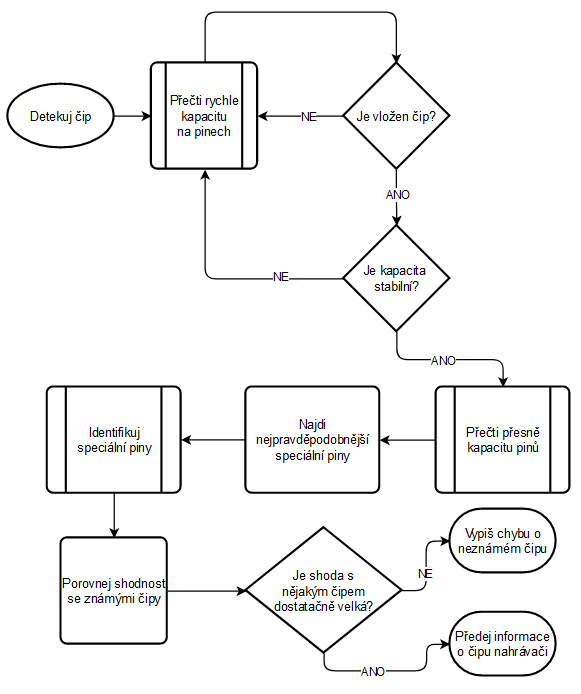
\includegraphics[width=0.75\linewidth]{img/detector_diagram.png}
  \centering
  \caption{Diagram fungování detektoru. Dvojité obdélníky značí funkce, které interagují s hardwarem}
  \label{fig:detector}
\end{figure}

Jednou z důležitých funkcí je detekce speciálních pinů. Pro každý pin vloženého čipu vyčíslíme, jak moc se relativně odlišuje od průměrné kapacity pinů na daném čipu. Toto číslo budeme přeneseně brát jako pravděpodobnost, že pin je speciálním pinem. Pět pinů\footnote{Nejvyšší počet speciálních pinů, který může AR čip o maximální podporované velikosti, je 5, včetně RESETu, ale teoreticky ani čip s více speciálními piny nebude problém detekovat, neboť i s pomocí pěti pinů bychom ho měli s jistotou určit.} s největší pravděpodobností vybereme a budeme je dále identifikovat, jak zachycuje obrázek \ref{fig:detect_special}.
Vzhledem k zjištěním při měření kapacity popsaných v sekci \ref{software:capacitance} by se mělo jednat, s danou pravděpodobností, o některý ze speciálních pinů - tedy buď GND, VCC nebo RESET.

\begin{figure}
  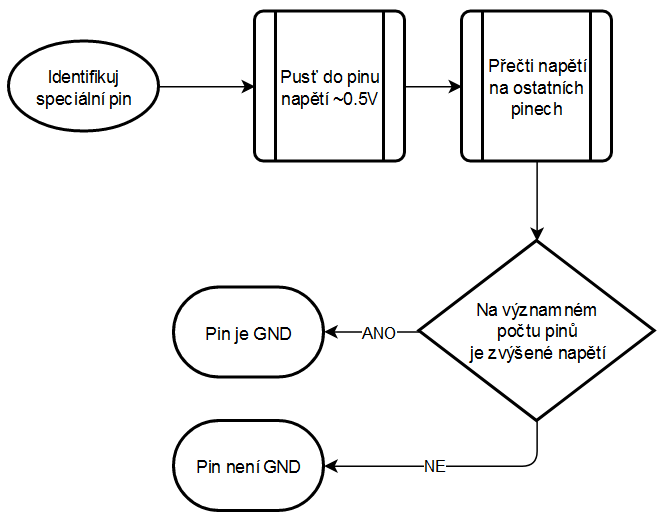
\includegraphics[width=0.6\linewidth]{img/identify_special_diagram.png}
  \centering
  \caption{Diagram identifikace speciálních pinů}
  \label{fig:detect_special}
\end{figure}

Cílem identifikace je rozpoznat, jestli je speciální pin GND. Ke pět nejpravděpodobnějším speciálním pinům, které jsme vybrali, si doplníme informaci jestli jsou pinem GND. Pokud pin není GND, jedná se buď o VCC, RESET, nebo o pin, který byl chybně detekován jako speciální (v takovém případě by jeho pravděpodobnost, a tedy i vliv na výslednou volbu čipu, měla být minimální).

Nakonec budeme iterovat přes všechny podporované čipy dané velikosti a pro obě možná otočení čipu zjistíme, jestli jeho speciální piny sedí se speciálními piny, které jsme detekovali. Výsledná shoda čipu je součet pravděpodobností těchto shodných speciálních pinů. Nejpravděpodobnější čip, který překonal stanovenou minimální shodu, je prohlášen za identifikovaný a informace o něm jsou předány dále.

\subsection {Nahrávač \label{software:uploader}}

Díky detektoru teď víme, jaký čip je vložen do patice, na jaké je pozici a jak je orientovaný. Víme tedy také, kde jsou umístěny piny, které potřebujeme pro nahrávání. Tyto informace již tedy stačí předat nahrávači. Pro zjednodušení jsem využil již implementovaný nahrávač, Arduino ISP, který je distribuovaný s Arduino IDE. Tento nahrávač jsem zvolil mimo jiné proto, že ho lze snadno ovládat právě z Arduino IDE a při použití USP uživatelem tedy nebude nutné nic instalovat ani upravovat.

Do Arduino ISP jsem doimplementoval softwarový oscilátor pomocí hardwarového časovače zabudovaného v čipu ATmega2560 \cite{atmega2560}. Díky tomu je možné programovat i čipy, které vyžadují externí oscilátor.

Implementace nahrávače je udělaná tak, aby ho v případě potřeby bylo možné snadno vyměnit za jiný. To bude nutné třeba pro přidání podpory HVSP či HVPP, neboť tyto protokoly Arduino ISP nepodporuje.

\chapter{Technická dokumentace}

\section {Použití}

Univerzální sériový programátor nevyžaduje instalaci žádného dalšího programu pro použití. Z vnějšího pohledu se chová stejně jako standardní Arduino ISP, které je široce podporované. Po zapojení do počítače přes USB type-B port, kterým je Arduino Mega vybaveno, může chvíli (několik sekund) trvat, než se USP inicializuje a zahájí komunikaci s počítačem přes sériový port\footnote{Ke komunikaci je nutné mít ovladače, ty se ale nainstalují samy při instalaci Arduina IDE, AVRDUDE nebo podobných programů.}. Poté, co se na obrazovce USP objeví nápis \lq Ready\rq ,  je USP připraven k vložení čipu. Ten může být vložen s libovolnou orientací a na libovolné místo. Aktuální verze USP podporuje prakticky všechny čipy řad Atmega a ATtiny v provedení DIP.\footnote{Fyzicky jsem však testoval jen dva různé čipy ATtiny a jeden ATmega, takže je možné, že pro určité specifické čipy bude potřeba upravit parametry v kódu a ten flashovat do USP, více o tom v sekci \ref{selfupload}.} 

Ihned po vložení čipu a jeho zajištění páčkou probíhá detekování. Během tohoto procesu se programátoru nedotýkejte, mohlo by to způsobit špatnou detekci čipu. Po detekování se na displeji ukáže jméno detekovaného čipu.\footnote{Jméno na displeji se může lišit od reálného použitého čipu, neboť existuje mnoho variant čipů se stejným rozložením. Na displeji je zobrazeno jméno nejznámnějšího čipu s daným rozložením nebo čipu s největší pamětí.} V této chvíli je již možné do čipu nahrávat stejným způsobem jako do normálního zařízení Arduino ISP. Možné způsoby nahrávání do čipů přes USP si rozebereme v následujích sekcích.

Po vyndání čipu je možné stiskem libovolného tlačítka resetovat USP do původního stavu a připravit ho na další čip, který je možné vložit poté, co se na displeji objeví \lq Ready\rq .

\subsection {Použití s Arduino IDE}

Použití s Arduino IDE je pravděpodobně nejjednodušší. Jako příklad řekněme, že chceme nahrát program do čipu Atmega328P, který mimo jiné pohání Arduino Uno. Prvním krokem je zvolit Arduino ISP jako programátor pod Nástroje>Programátor>Arduino as ISP a zvolit Port do kterého je USP připojen. V nabídce portů se bude USP ukazovat pod jménem Arduino Mega. Dalším krokem je zvolit čip, do kterého budeme nahrávat v Nástroje>Vývojová deska. V našem příkladě to bude \lq Arduino Uno\rq , pod čímž se skrývá čip Atmega328 nastavený na použití externího oscilátoru s frekvencí 16Mhz, který je na desce Arduino Uno. Toto nastavení, se zvýrazněnými důležitými parametry, je na obrázku \ref{fig:uno_settings}.

\begin{figure}[ht!]
  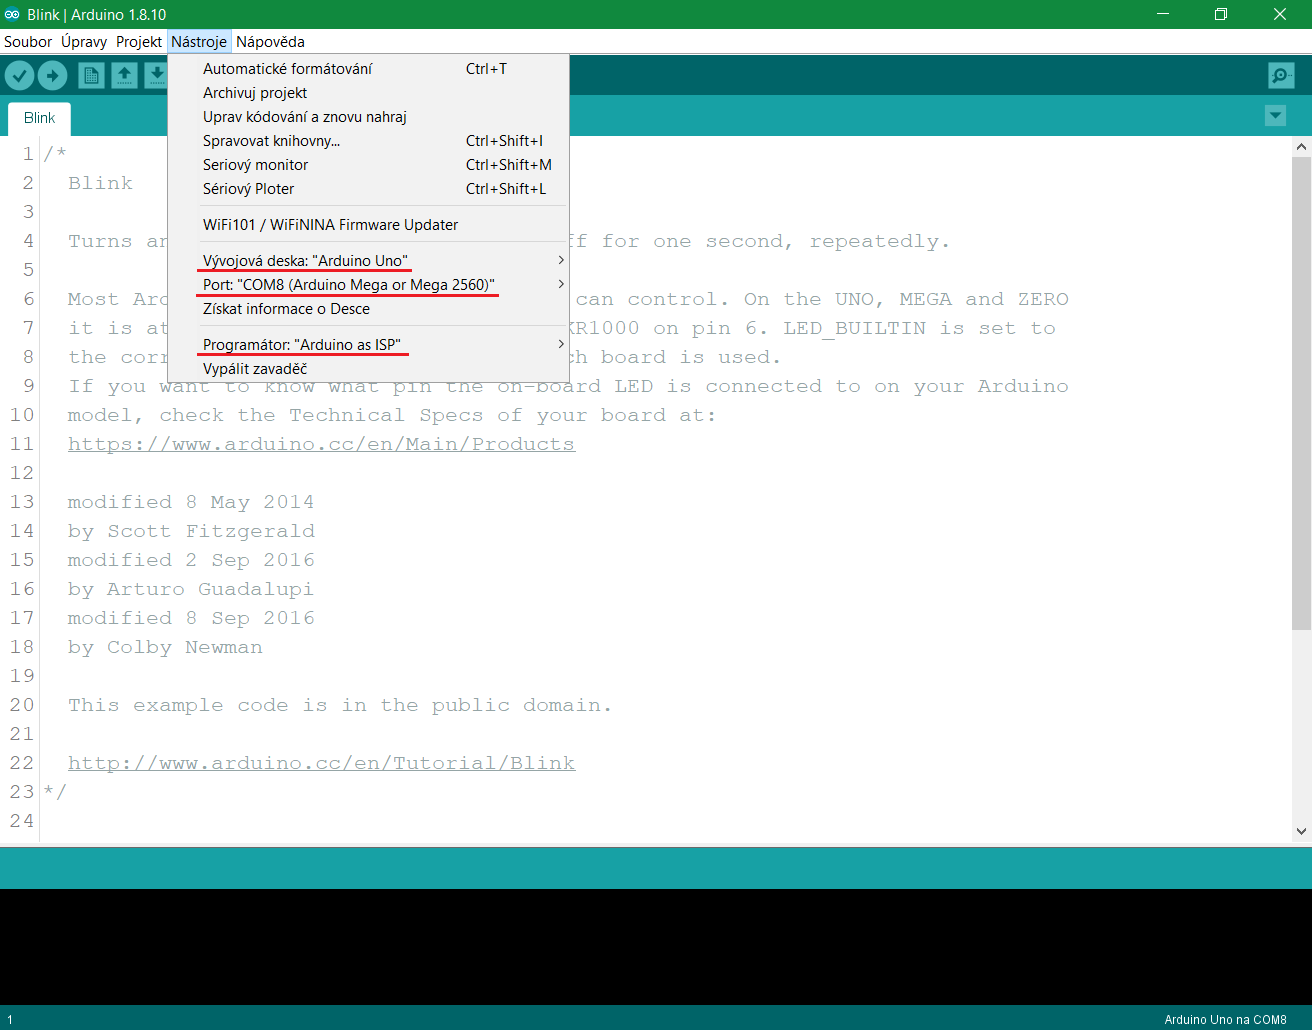
\includegraphics[width=\linewidth]{img/uno_settings.png}
  \centering
  \caption{Nastavení Arduino IDE pro nahrávání do čipu ATmega328 s externím oscilátorem 16Mhz; zvýrazněny jsou nejdůležitější parametry.}
  \label{fig:uno_settings}
\end{figure}

Nahrávání do jiných mikrokontrolérů, kterými nejsou obsazeny desky Arduino, vyžaduje stažení příslušných knihoven. Pro čipy ATtiny může být použita například knihovna ATTinyCore \cite{attinycore}. Po jejím nainstalování se nám příslušné mikrokontroléry ukáží pod Nástroje>Vývojová deska a bude pro ně dostupné více nastavení. Možná nastavení, která nemusí být dostupná pro každý mikrokontrolér, jsou BOD (Brown-out detection; napětí, při kterém se čip vypně), číslování pinů, hodiny (vnitřní/vnější oscilátor a jeho frekvence) a mnoho dalšího. Příklad nastavení pro programování čipu ATtiny84 s interním oscilátorem 8Mhz je na obrázku \ref{fig:attiny84_settings}.

\begin{figure}[ht!]
  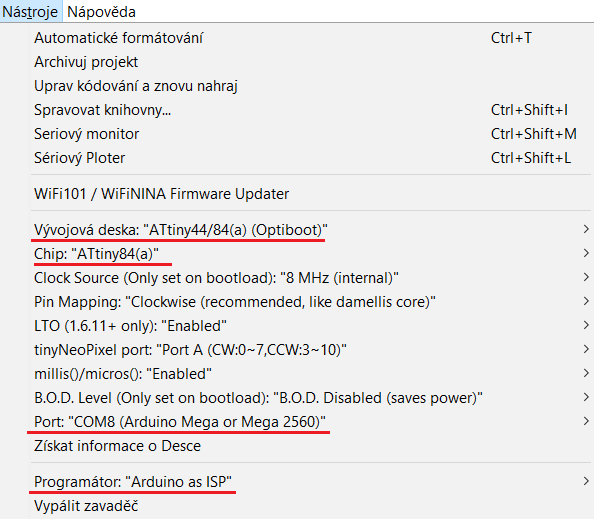
\includegraphics[width=0.6\linewidth]{img/settings.png}
  \centering
  \caption{Nastavení Arduino IDE pro nahrávání do čipu ATtiny84; zvýrazněny jsou nejdůležitější parametry.}
  \label{fig:attiny84_settings}
\end{figure}


V případě, že je toto první nahrávání do konkrétního čipu bude potřeba vypálit bootloader. To lze v Arduino IDE udělat pod Nástroje>Vypálit zavaděč. Tím se příslušné parametry, jako frekvence oscilátoru či BOD, vypálí do mikrokontroléru. Poté je již možné nahrávat program do čipu pod Projekt>Nahrát pomocí programátoru nebo pomocí zkratky Ctrl+Shift+U. 

Mikrokontrolér, do kterého jsme nahrávali kód pomocí programátoru, nebude následně možné programovat pomocí sériového portu. Tento způsob programování je využíván například při bězném nahrávání do desek Arduino Uno. Pokud tedy chceme čip vložit do desky Arduino Uno nebo podobné, bude nutné znovu vypálit bootloader pod Nástroje>Vypálit zavaděč. Poté již do čipu nenahrávejte s pomocí USP a vložte jej do desky Arduino Uno.

\subsection {Použití s AVRDUDE}

\begin{figure}[ht!]
  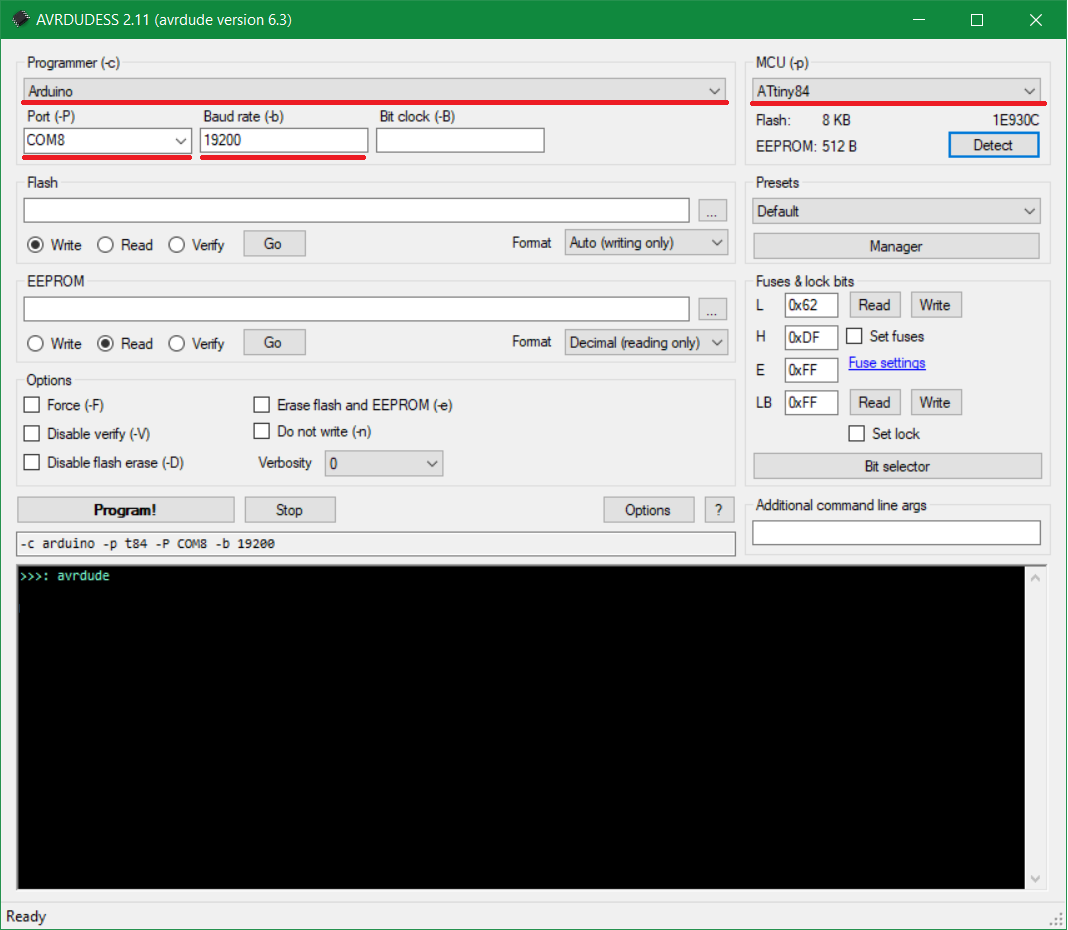
\includegraphics[width=\linewidth]{img/avrdude.png}
  \centering
  \caption{Nastavení AVRDUDESS pro nahrávání do čipu Attiny84, zvýrazněny jsou nejdůležitější parametry.}
  \label{fig:avrdude}
\end{figure}

Podobně jako s Arduino IDE, lze nahrávat i programem AVRDUDE, případně s použitím UI verze zvané AVRDUDESS. Opět je nutné pouze zvolit port, programátor Arduino, cílový čip a tentokrát i rychlost komunikace 19200 baudů. Nastavení pro ATtiny84 je dostupné na obrázku \ref{fig:avrdude}. Hlavní výhodou AVRDUDE je, že pomocí něj jsme schopni nastavovat a číst fuse bits, číst a zapisovat do EEPROM či flash paměti či nastavovat lock bits. Lze pomocí něj do určité míry oživovat i zdánlivě mrtvé čipy.

\section {Nahrávání od USP \label{selfupload}}

Deska USP chrání řídící mikroprocesor na Arduino Mega proti nechtěnému flashování. V případě, že bude potřeba do něj nahrávat, je nutné nejdříve odstranit žlutý jumper s označením \lq self prog\rq , který se nachází na druhé straně desky než displej a tlačítka. Poté bude již možné nahrávat do Arduino Mega standardním způsobem.

\chapter*{Závěr}
\pagestyle{empty}
\addcontentsline{toc}{chapter}{Závěr}

Hlavním cílem projektu bylo vytvořit hardwarový výrobek, který bude reálně užitečný a výrazně zjednodušší nahrávání do (převážně) AVR čipů v pouzdře DIP. Tento cíl projekt splnil. Na hardwarové úrovni bylo implementováno i několik bonusových funkcí, jako například podpora vysokonapěťového programování, které pouze čekají na implementaci v softwaru.

Zařízení je funkční a bylo otestováno na několika mikrokontrolérech, které jsem měl k dispozici. Jeho spolehlivost by bylo možné dále zvýšit důkladnějším testování na dalších čipech a doladěním parametrů detekce. Také by bylo možné vytvořit uživatelsky přívětivé rozhraní, které by umožňovalo například volbu nahrávacího protokolu, případně poskytovalo některé funkce i bez připojení k počítači, k čemuž je také připraven potřebný hardware.

Během práce na projektu jsem se toho mnoho naučil nejen o AVR čipech a CMOS obvodech, které jsem využíval, ale také o elektrotechnice obecně. Získal jsem cenné zkušeností při návrhu plošného spoje, výběru potřebných komponent a zkoumání jejich vzájemných interakcí.  


%%% Seznam použité literatury
\printbibliography[title={Seznam použité literatury},heading={bibintoc}]

%%% Seznam obrázků
\openright
\listoffigures
\addcontentsline{toc}{chapter}{Seznam obrázků}

%%% Přílohy k práci, existují-li. Každá příloha musí být alespoň jednou
%%% odkazována z vlastního textu práce. Přílohy se číslují.

\part*{Přílohy}
\appendix

\renewcommand{\thefigure}{A.\arabic{figure}}

\setcounter{figure}{0}

\begin{figure}[ht!]
  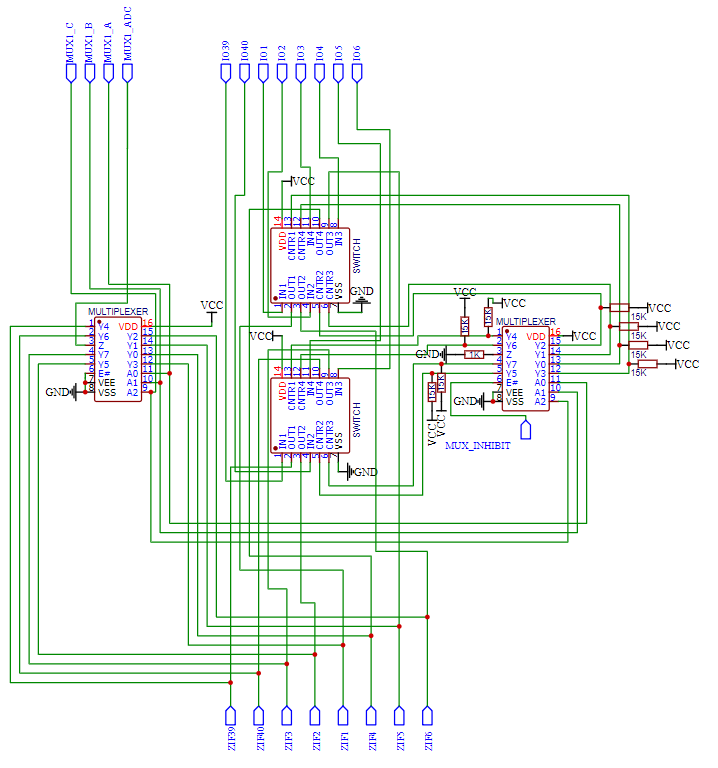
\includegraphics[width=\linewidth]{img/pin_switches.png}
  \centering
  \caption{Úplné schéma obvodu připojeného k 8 pinům ZIF patice.}
  \label{appendix:pin_switches}
\end{figure}

\begin{figure}[ht!]
  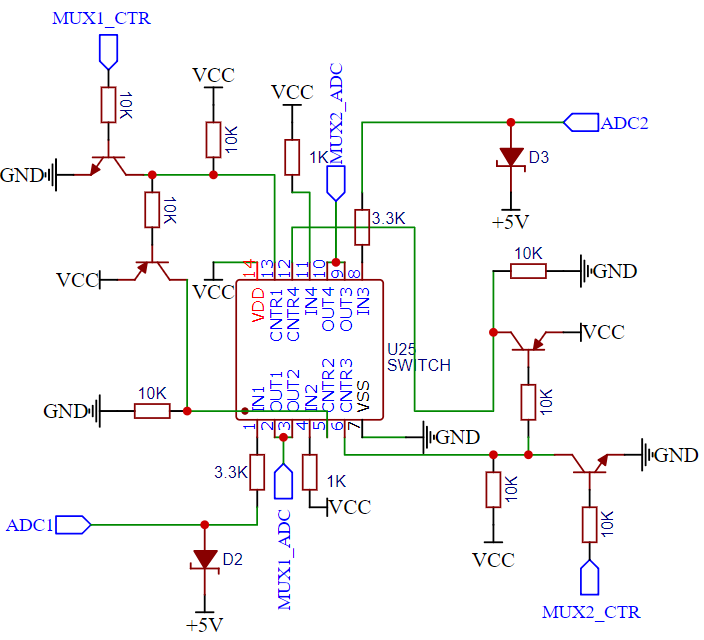
\includegraphics[width=\linewidth]{img/mux_input_control.png}
  \centering
  \caption{Úplné schéma zapojení switche, který přepíná vstup do multiplexerů 1 a 2 mezi ADC pinem a 12V.}
  \label{appendix:mux_input_control}
\end{figure}

\begin{figure}[ht!]
  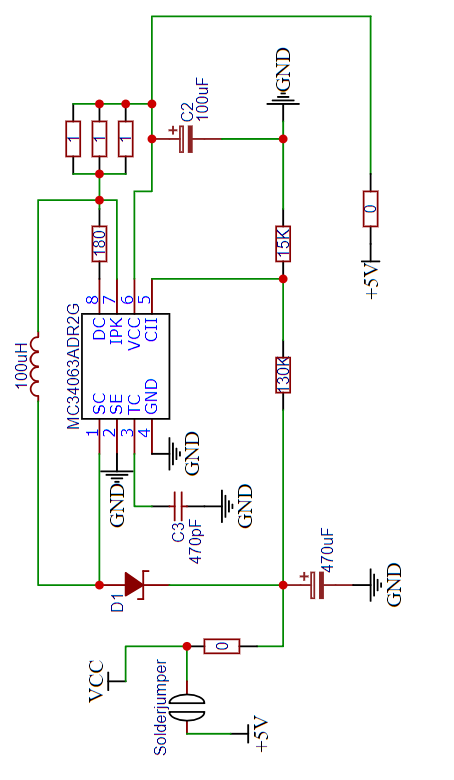
\includegraphics[width=0.8\linewidth]{img/boost_converter.png}
  \centering
  \caption{Úplné schéma obvodu step-up převodníku z 5 na 12 voltů. Obvod zahrnuje nula ohmové odpory a solder jumper, které umožňují jednoduché odpojení převodníku.}
  \label{appendix:boost_converter}
\end{figure}

\begin{figure}[ht!]
  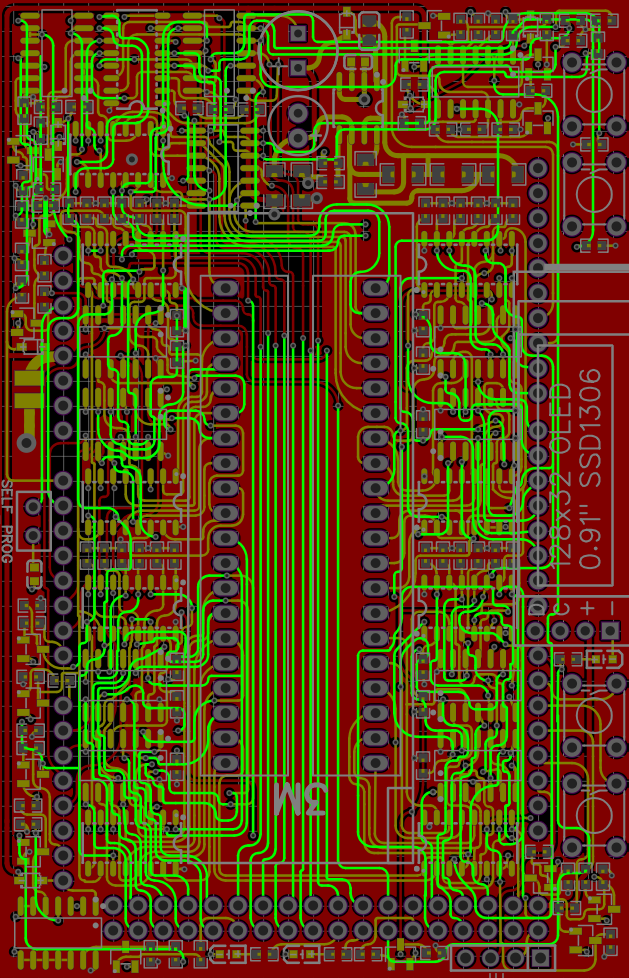
\includegraphics[width=\linewidth]{img/board.png}
  \centering
  \caption{Zapojení plošného spoje. Žlutou barvou jsou vyznačeny spoje ve vrchní vrstvě, zelenou spoje spodní vrstvy a červenou spoje jedné z vnitřních vrstev. Druhá vnitřní vrstva není na obrázku zachycena.}
  \label{appendix:board}
\end{figure}

\end{document}
